% Options for packages loaded elsewhere
\PassOptionsToPackage{unicode}{hyperref}
\PassOptionsToPackage{hyphens}{url}
%
\documentclass[
  12pt,
]{article}
\title{Exploring the Determinants of Biogas Generation Potential in
California}
\usepackage{etoolbox}
\makeatletter
\providecommand{\subtitle}[1]{% add subtitle to \maketitle
  \apptocmd{\@title}{\par {\large #1 \par}}{}{}
}
\makeatother
\subtitle{Web address for GitHub repository}
\author{Jibikeoluwa Faborode, Yinan Ding, Abhay Rao}
\date{}

\usepackage{amsmath,amssymb}
\usepackage{lmodern}
\usepackage{iftex}
\ifPDFTeX
  \usepackage[T1]{fontenc}
  \usepackage[utf8]{inputenc}
  \usepackage{textcomp} % provide euro and other symbols
\else % if luatex or xetex
  \usepackage{unicode-math}
  \defaultfontfeatures{Scale=MatchLowercase}
  \defaultfontfeatures[\rmfamily]{Ligatures=TeX,Scale=1}
  \setmainfont[]{Times New Roman}
\fi
% Use upquote if available, for straight quotes in verbatim environments
\IfFileExists{upquote.sty}{\usepackage{upquote}}{}
\IfFileExists{microtype.sty}{% use microtype if available
  \usepackage[]{microtype}
  \UseMicrotypeSet[protrusion]{basicmath} % disable protrusion for tt fonts
}{}
\makeatletter
\@ifundefined{KOMAClassName}{% if non-KOMA class
  \IfFileExists{parskip.sty}{%
    \usepackage{parskip}
  }{% else
    \setlength{\parindent}{0pt}
    \setlength{\parskip}{6pt plus 2pt minus 1pt}}
}{% if KOMA class
  \KOMAoptions{parskip=half}}
\makeatother
\usepackage{xcolor}
\IfFileExists{xurl.sty}{\usepackage{xurl}}{} % add URL line breaks if available
\IfFileExists{bookmark.sty}{\usepackage{bookmark}}{\usepackage{hyperref}}
\hypersetup{
  pdftitle={Exploring the Determinants of Biogas Generation Potential in California},
  pdfauthor={Jibikeoluwa Faborode, Yinan Ding, Abhay Rao},
  hidelinks,
  pdfcreator={LaTeX via pandoc}}
\urlstyle{same} % disable monospaced font for URLs
\usepackage[margin=2.54cm]{geometry}
\usepackage{graphicx}
\makeatletter
\def\maxwidth{\ifdim\Gin@nat@width>\linewidth\linewidth\else\Gin@nat@width\fi}
\def\maxheight{\ifdim\Gin@nat@height>\textheight\textheight\else\Gin@nat@height\fi}
\makeatother
% Scale images if necessary, so that they will not overflow the page
% margins by default, and it is still possible to overwrite the defaults
% using explicit options in \includegraphics[width, height, ...]{}
\setkeys{Gin}{width=\maxwidth,height=\maxheight,keepaspectratio}
% Set default figure placement to htbp
\makeatletter
\def\fps@figure{htbp}
\makeatother
\setlength{\emergencystretch}{3em} % prevent overfull lines
\providecommand{\tightlist}{%
  \setlength{\itemsep}{0pt}\setlength{\parskip}{0pt}}
\setcounter{secnumdepth}{5}
\ifLuaTeX
  \usepackage{selnolig}  % disable illegal ligatures
\fi

\begin{document}
\maketitle

\newpage
\tableofcontents 
\newpage
\listoftables 
\newpage
\listoffigures 


\newpage

\hypertarget{table-of-figures}{%
\section{Table of figures}\label{table-of-figures}}

Figure 1: Population density across counties im California

Figure 2: Impoverished population density across counties in California

Figure 3: Total Methane potential across counties in California

Figure 4: Waste water Methane Potential across counties in California

Figure 5: Landfill methane potential across counties in California

Figure 6: Organic Waste methane potential across counties in California

Figure 7: Animal manure methane potential across counties in California

Figure 8:

Figure 9:

Figure 10:

Figure 11:

Figure 12:

Figure 13:

Figure 14:

\newpage

\hypertarget{background}{%
\section{Background}\label{background}}

\hypertarget{rationale-of-the-study}{%
\subsection{Rationale of the study}\label{rationale-of-the-study}}

The transition to cleaner and renewable sources of energy requires more
work to scale already existing gains, for example in the area of biogas
utilization, while also seeking out new opportunities. Biogas is a form
of renewable energy produced by anaerobic decomposition or
thermochemical conversion of biomass such as agricultural waste, manure,
municipal waste sewage, green waste and food waste. Biogas is composed
mostly of methane, alongside carbon dioxide, water vapor and other
gases. Similar to natural gas, biogas can be burned directly as a fuel
or treated to remove the CO2 and other gases before for being used in
the form of biomethane.

Utilizing biogas as an energy source helps to transform harmful gases
from decomposing waste into positive use. Methane is a powerful
greenhouse gas that traps heat in the atmosphere, with a global warming
potential estimated to be over 25 times as potent as that of Carbon
Dioxide.Transforming waste into biogas therefore reduces greenhouse gas
emissions and the risk of pollution to waterways. The
\href{https://unece.org/challenge\#:~:text=Methane\%20is\%20a\%20powerful\%20greenhouses,grows\%20to\%2084\%2D86\%20times.}{UNECE}
estimates that over a 20 year period, this ratio increases to 84-86
times. However, stored biogas limits the amount of methane released into
the atmosphere and reduces dependence on fossil fuels. When stored ,
biogas serves as a renewable and reliable baseload power source and can
even be used to rapidly meet peak power demands. When biogas is used for
energy generation in place of fossil fuels, it enables even more
emission reductions, sometimes resulting in carbon negative systems.
According to the
\href{https://www.eesi.org/papers/view/fact-sheet-biogasconverting-waste-to-energy}{Environmental
and Energy Study Institute, EESI} ,the reduction of methane emissions
derived from tapping all the potential biogas in the United States would
be equal to the annual emissions of 800,000 to 11 million passenger
vehicles.

Unfortunately, despite the various benefits offered by biogas energy,
the United States currently only has 2,200 operating biogas systems. The
EESI estimates this current capacity to be less than 20\% of the total
potential. It is on this basis that this study attempts to examine the
factors contributing to biogas generation potential, particularly in
California. California was selected because of its status as a leading
state in biogas generation potential based on estimates by the National
Renewable Energy Laboratory (NREL). According to the
\href{chrome-extension://efaidnbmnnnibpcajpcglclefindmkaj/viewer.html?pdfurl=https\%3A\%2F\%2Famericanbiogascouncil.org\%2Fwp-content\%2Fuploads\%2F2019\%2F05\%2FABCBiogasStateProfile_CA.pdf\&clen=226298\&chunk=true}{American
Biogas Council}, California can power nearly 200,000 homes if this
biogas is utilized appropriately. The results of our analysis for
California can provide the basis for further analysis across several
other US states.

\hypertarget{research-questions}{%
\subsection{Research Questions}\label{research-questions}}

The analysis conducted was done based on two research questions:

\begin{enumerate}
\def\labelenumi{\arabic{enumi}.}
\item
  Is biogas generation potential correlated with population density
  across California counties?
\item
  What additional factors must be considered in determining biogas
  generation potential?
\end{enumerate}

\newpage

\hypertarget{dataset-information}{%
\section{Dataset Information}\label{dataset-information}}

the datasets used include the following:

\begin{enumerate}
\def\labelenumi{\arabic{enumi}.}
\item
  Methane Generation Potential The NREL's dataset on methane generation
  potential covers data for the entire United States of America. It
  particularly providing information for Methane generation potential
  across all states in metric tons from sources which include landfills,
  industrial organic waste, animal manure, and wastewater . All of these
  individual sources were aggregated to estimate total methane
  generation potential by state. The dataset contained estimates for
  2009 to 2012, being the latest available data we could find online.
\item
  Population data Population data was pulled from the latest available
  the Social Vulnerability Index data compiled by the Center for Disease
  Control (CDC) and Agency for Toxic Substance and Diseace Reegistry
  (ATSDR). This dataset also includes details on impoverished
  populations and spans from 2017-2018. Since the SDI offers data that
  helps to effectly plan towards meeting the needs of improverished
  populations, this dataset also helps to dds another dimension to our
  analysis as it enables the exploration of impacts on socially
  vulnerable people.
\end{enumerate}

\newpage

\hypertarget{exploratory-analysis}{%
\section{Exploratory Analysis}\label{exploratory-analysis}}

The two datasets were wrangled and joined both datasets to have a
unified dataframe that captured data on methane generation potential,
population and poverty levels by county. An initial exploration of the
data was done to provide a visual assessment of spatial data and
determine the emergence of any any trends.

\begin{verbatim}
## Simple feature collection with 6 features and 14 fields
## Geometry type: MULTIPOLYGON
## Dimension:     XY
## Bounding box:  xmin: -122.7851 ymin: 37.45447 xmax: -119.5423 ymax: 40.15203
## Geodetic CRS:  WGS 84
##   ObjectID      NAME STATE_NAME  FIPS      OWCH4t    AMCH4t     WWTPCH4t
## 1      184   Alameda California 06001 5700.695190  0.367359 10461.687700
## 2      185    Alpine California 06003    6.483819  0.000000     6.667176
## 3      186    Amador California 06005  156.310667  3.826180   624.136548
## 4      187     Butte California 06007  817.909133 20.460013  1210.759120
## 5      188 Calaveras California 06009   97.664105 11.663426   200.148617
## 6      189    Colusa California 06011   72.199705  2.057210   104.007942
##   LFGCH4t   TotalCH4t    COUNTY                     LOCATION E_TOTPOP  E_POV
## 1   49311 65473.75020   Alameda   Alameda County, California  1643700 170884
## 2       0    13.15099    Alpine    Alpine County, California     1146    227
## 3       0   784.27340    Amador    Amador County, California    37829   3323
## 4       0  2049.12827     Butte     Butte County, California   227075  44410
## 5       0   309.47615 Calaveras Calaveras County, California    45235   5242
## 6       0   178.26486    Colusa    Colusa County, California    21464   2929
##   E_MINRTY                       geometry
## 1  1120309 MULTIPOLYGON (((-122.313 37...
## 2      468 MULTIPOLYGON (((-120.0726 3...
## 3     8066 MULTIPOLYGON (((-121.0276 3...
## 4    62685 MULTIPOLYGON (((-122.0573 3...
## 5     8330 MULTIPOLYGON (((-120.9955 3...
## 6    13792 MULTIPOLYGON (((-122.7851 3...
\end{verbatim}

Visually, the most populated area of California, given by the county
shaded yellow, Los Angeles, has the highest methane (CH4) generation
potential. The density of impoverished population appears to be
similarly distributed.

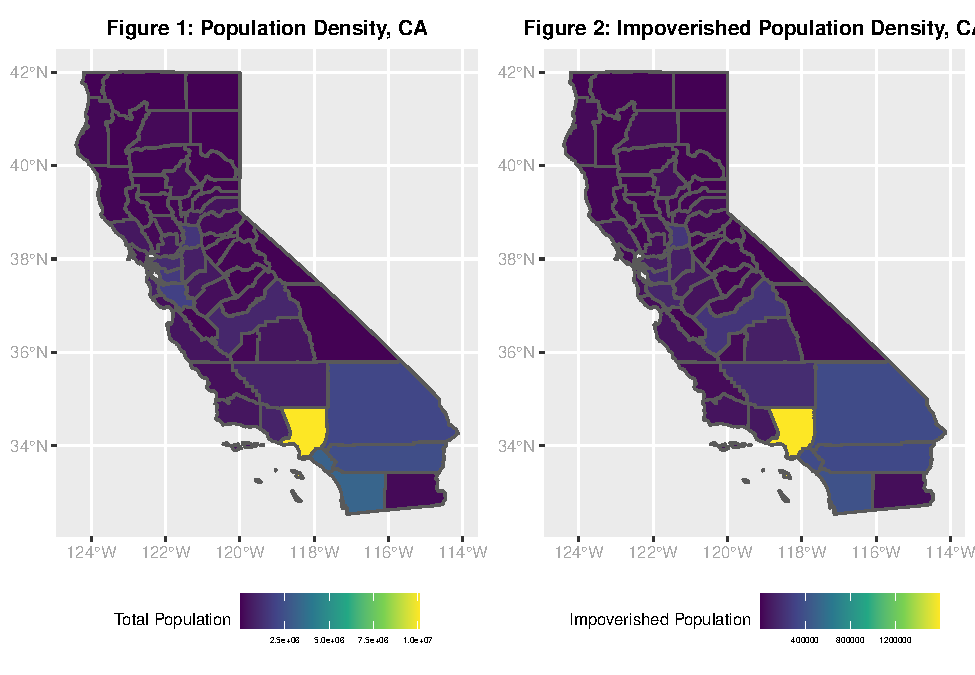
\includegraphics{FDR_ProjectReport_files/figure-latex/unnamed-chunk-3-1.pdf}
The total Methane generation potential is greatest at the most densely
populated areas. This trend appears to continue with wastewater derived
methane.

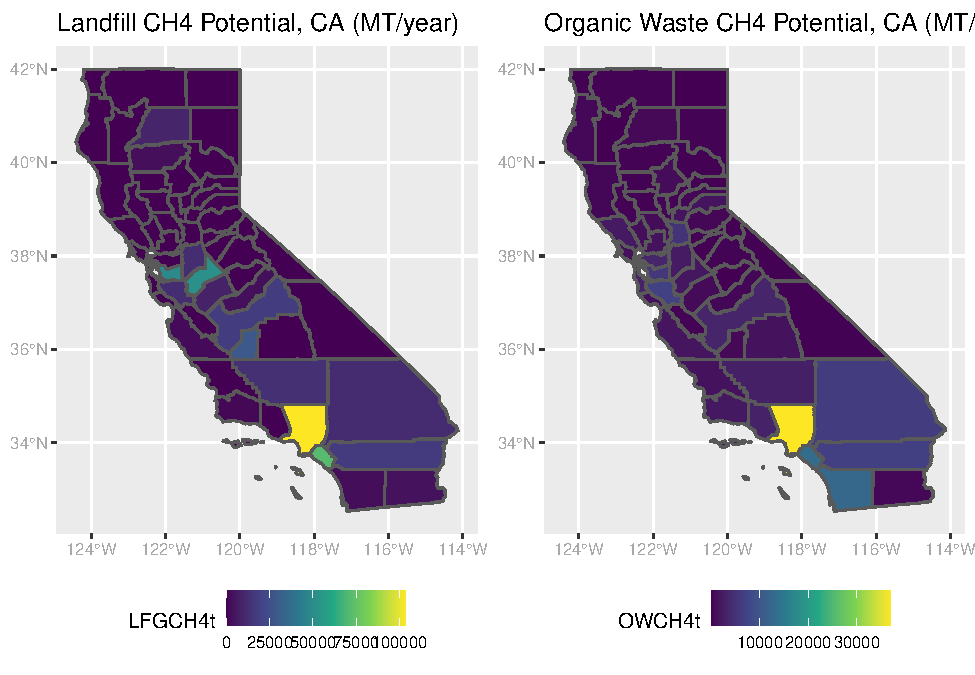
\includegraphics{FDR_ProjectReport_files/figure-latex/unnamed-chunk-4-1.pdf}

Industrial Organic waste, like wastewater, is highly correlated with
population.With landfill-based methane, some counties in central CA,
which do not appear to have a high population, have comparatively high
methane generation potential. There may be some non-population related
factors in play.
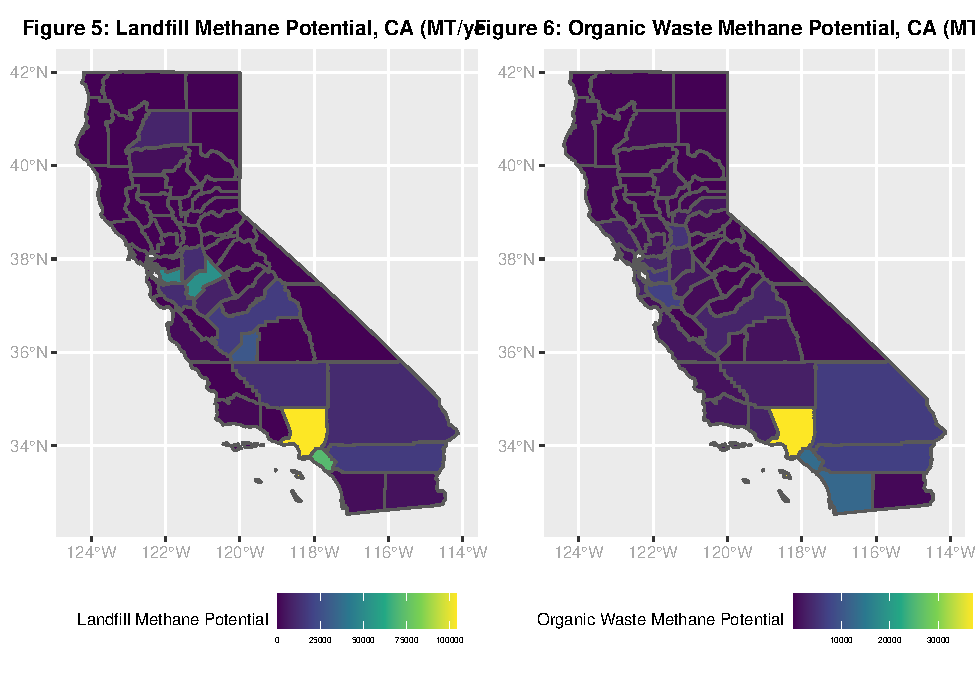
\includegraphics{FDR_ProjectReport_files/figure-latex/unnamed-chunk-5-1.pdf}

The trend with animal-manure derived CH4 however substantially differs
from the previous cases. Population does not appear to be a decisive
factor.

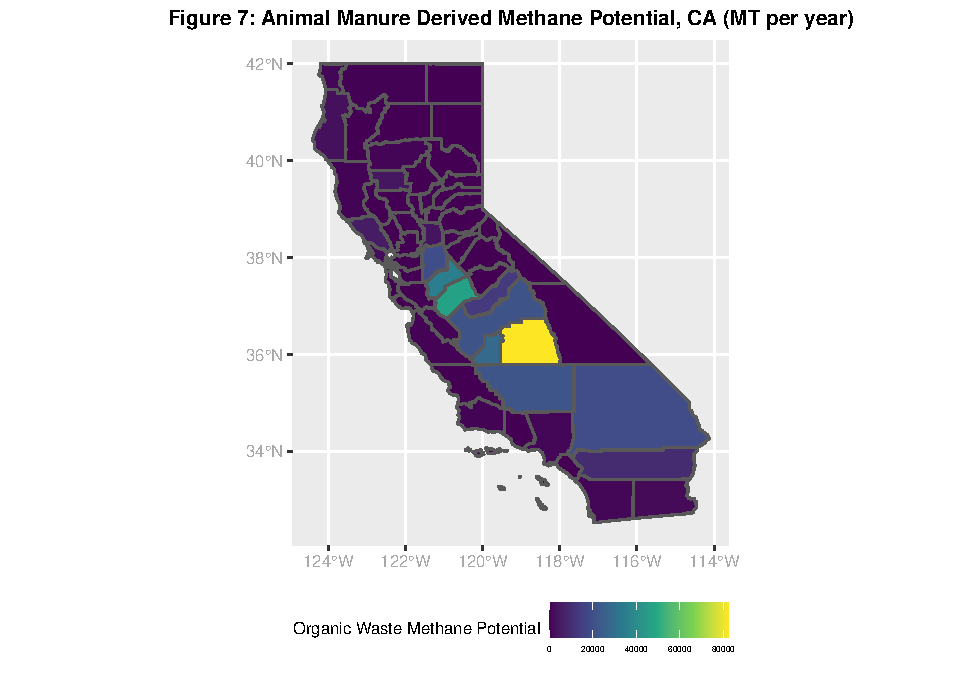
\includegraphics{FDR_ProjectReport_files/figure-latex/unnamed-chunk-6-1.pdf}

\newpage

\hypertarget{analysis}{%
\section{Analysis}\label{analysis}}

\hypertarget{question-1-insert-specific-question-here-and-add-additional-subsections-for-additional-questions-below-if-needed}{%
\subsection{Question 1: \textless insert specific question here and add
additional subsections for additional questions below, if
needed\textgreater{}}\label{question-1-insert-specific-question-here-and-add-additional-subsections-for-additional-questions-below-if-needed}}

\hypertarget{question-2-is-there-a-relationship-between-methane-generation-potential-and-impoverished-populations}{%
\subsection{Question 2: Is there a relationship between methane
generation potential and impoverished
populations?}\label{question-2-is-there-a-relationship-between-methane-generation-potential-and-impoverished-populations}}

\begin{verbatim}
## 
##  Pearson's product-moment correlation
## 
## data:  svi_sf_join$TotalCH4t and svi_sf_join$E_POV
## t = 11.12, df = 56, p-value = 8.476e-16
## alternative hypothesis: true correlation is not equal to 0
## 95 percent confidence interval:
##  0.7271725 0.8959424
## sample estimates:
##       cor 
## 0.8296405
\end{verbatim}

\begin{verbatim}
## 
## Call:
## lm(formula = svi_sf_join$TotalCH4t ~ svi_sf_join$E_POV)
## 
## Residuals:
##    Min     1Q Median     3Q    Max 
## -23578  -8007  -6799  -4377  74610 
## 
## Coefficients:
##                    Estimate Std. Error t value Pr(>|t|)    
## (Intercept)       6.684e+03  2.834e+03   2.358   0.0219 *  
## svi_sf_join$E_POV 1.310e-01  1.178e-02  11.120 8.48e-16 ***
## ---
## Signif. codes:  0 '***' 0.001 '**' 0.01 '*' 0.05 '.' 0.1 ' ' 1
## 
## Residual standard error: 19840 on 56 degrees of freedom
## Multiple R-squared:  0.6883, Adjusted R-squared:  0.6827 
## F-statistic: 123.7 on 1 and 56 DF,  p-value: 8.476e-16
\end{verbatim}

\begin{verbatim}
## 
##  Pearson's product-moment correlation
## 
## data:  svi_sf_join$LFGCH4t and svi_sf_join$E_POV
## t = 9.3128, df = 56, p-value = 5.653e-13
## alternative hypothesis: true correlation is not equal to 0
## 95 percent confidence interval:
##  0.6526255 0.8638755
## sample estimates:
##       cor 
## 0.7795177
\end{verbatim}

\begin{verbatim}
## 
## Call:
## lm(formula = svi_sf_join$LFGCH4t ~ svi_sf_join$E_POV)
## 
## Residuals:
##    Min     1Q Median     3Q    Max 
## -24928  -3488  -1556  -1095  47103 
## 
## Coefficients:
##                    Estimate Std. Error t value Pr(>|t|)    
## (Intercept)       1.059e+03  1.700e+03   0.623    0.536    
## svi_sf_join$E_POV 6.581e-02  7.067e-03   9.313 5.65e-13 ***
## ---
## Signif. codes:  0 '***' 0.001 '**' 0.01 '*' 0.05 '.' 0.1 ' ' 1
## 
## Residual standard error: 11900 on 56 degrees of freedom
## Multiple R-squared:  0.6076, Adjusted R-squared:  0.6006 
## F-statistic: 86.73 on 1 and 56 DF,  p-value: 5.653e-13
\end{verbatim}

\begin{verbatim}
## 
##  Pearson's product-moment correlation
## 
## data:  svi_sf_join$WWTPCH4t and svi_sf_join$E_POV
## t = 30.671, df = 56, p-value < 2.2e-16
## alternative hypothesis: true correlation is not equal to 0
## 95 percent confidence interval:
##  0.9521271 0.9831025
## sample estimates:
##       cor 
## 0.9715012
\end{verbatim}

\begin{verbatim}
## 
## Call:
## lm(formula = svi_sf_join$WWTPCH4t ~ svi_sf_join$E_POV)
## 
## Residuals:
##     Min      1Q  Median      3Q     Max 
## -8111.2  -525.9  -266.3   200.7  8372.5 
## 
## Coefficients:
##                    Estimate Std. Error t value Pr(>|t|)    
## (Intercept)       2.329e+02  2.977e+02   0.782    0.437    
## svi_sf_join$E_POV 3.795e-02  1.237e-03  30.671   <2e-16 ***
## ---
## Signif. codes:  0 '***' 0.001 '**' 0.01 '*' 0.05 '.' 0.1 ' ' 1
## 
## Residual standard error: 2084 on 56 degrees of freedom
## Multiple R-squared:  0.9438, Adjusted R-squared:  0.9428 
## F-statistic: 940.7 on 1 and 56 DF,  p-value: < 2.2e-16
\end{verbatim}

\begin{verbatim}
## 
##  Pearson's product-moment correlation
## 
## data:  svi_sf_join$OWCH4t and svi_sf_join$E_POV
## t = 34.256, df = 56, p-value < 2.2e-16
## alternative hypothesis: true correlation is not equal to 0
## 95 percent confidence interval:
##  0.9612260 0.9863552
## sample estimates:
##       cor 
## 0.9769612
\end{verbatim}

\begin{verbatim}
## 
## Call:
## lm(formula = svi_sf_join$OWCH4t ~ svi_sf_join$E_POV)
## 
## Residuals:
##     Min      1Q  Median      3Q     Max 
## -2379.5  -363.1  -195.7    96.0  4351.1 
## 
## Coefficients:
##                    Estimate Std. Error t value Pr(>|t|)    
## (Intercept)       1.895e+02  1.656e+02   1.144    0.257    
## svi_sf_join$E_POV 2.359e-02  6.885e-04  34.256   <2e-16 ***
## ---
## Signif. codes:  0 '***' 0.001 '**' 0.01 '*' 0.05 '.' 0.1 ' ' 1
## 
## Residual standard error: 1160 on 56 degrees of freedom
## Multiple R-squared:  0.9545, Adjusted R-squared:  0.9536 
## F-statistic:  1174 on 1 and 56 DF,  p-value: < 2.2e-16
\end{verbatim}

\begin{verbatim}
## 
##  Pearson's product-moment correlation
## 
## data:  svi_sf_join$AMCH4t and svi_sf_join$E_POV
## t = 0.43506, df = 56, p-value = 0.6652
## alternative hypothesis: true correlation is not equal to 0
## 95 percent confidence interval:
##  -0.2033043  0.3116628
## sample estimates:
##        cor 
## 0.05803922
\end{verbatim}

\begin{verbatim}
## 
## Call:
## lm(formula = svi_sf_join$AMCH4t ~ svi_sf_join$E_POV)
## 
## Residuals:
##    Min     1Q Median     3Q    Max 
## -10228  -5295  -5206  -3608  76704 
## 
## Coefficients:
##                    Estimate Std. Error t value Pr(>|t|)  
## (Intercept)       5.202e+03  2.023e+03   2.572   0.0128 *
## svi_sf_join$E_POV 3.658e-03  8.408e-03   0.435   0.6652  
## ---
## Signif. codes:  0 '***' 0.001 '**' 0.01 '*' 0.05 '.' 0.1 ' ' 1
## 
## Residual standard error: 14160 on 56 degrees of freedom
## Multiple R-squared:  0.003369,   Adjusted R-squared:  -0.01443 
## F-statistic: 0.1893 on 1 and 56 DF,  p-value: 0.6652
\end{verbatim}

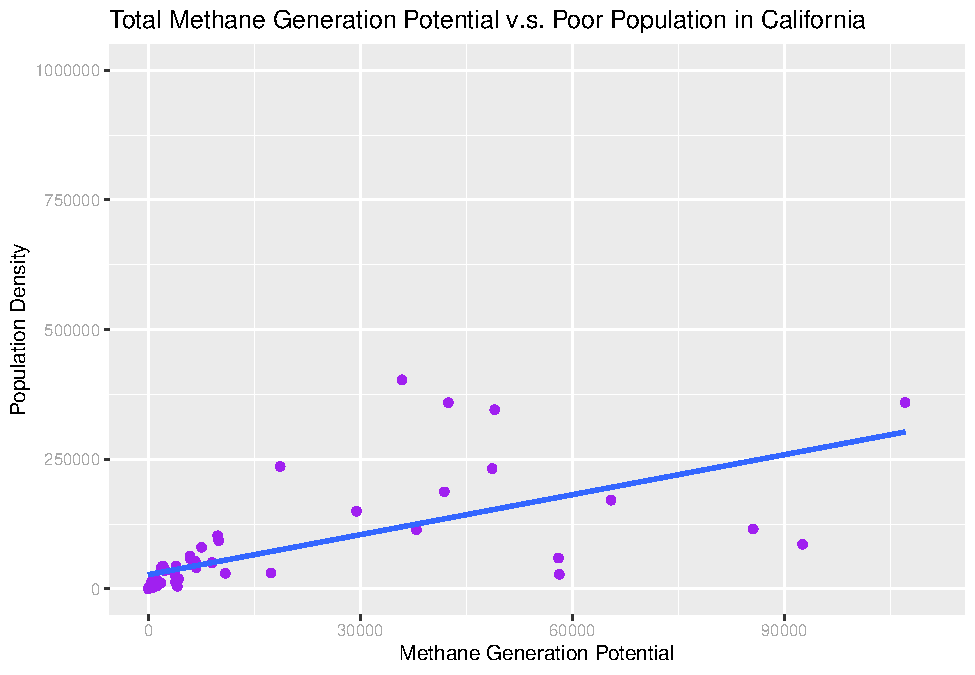
\includegraphics{FDR_ProjectReport_files/figure-latex/unnamed-chunk-8-1.pdf}
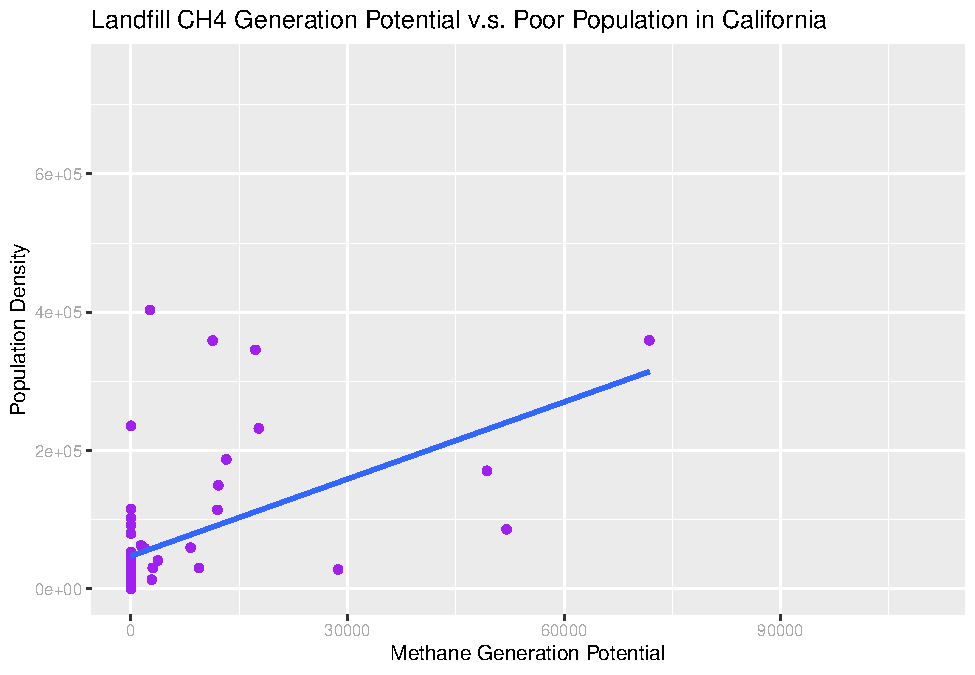
\includegraphics{FDR_ProjectReport_files/figure-latex/unnamed-chunk-8-2.pdf}
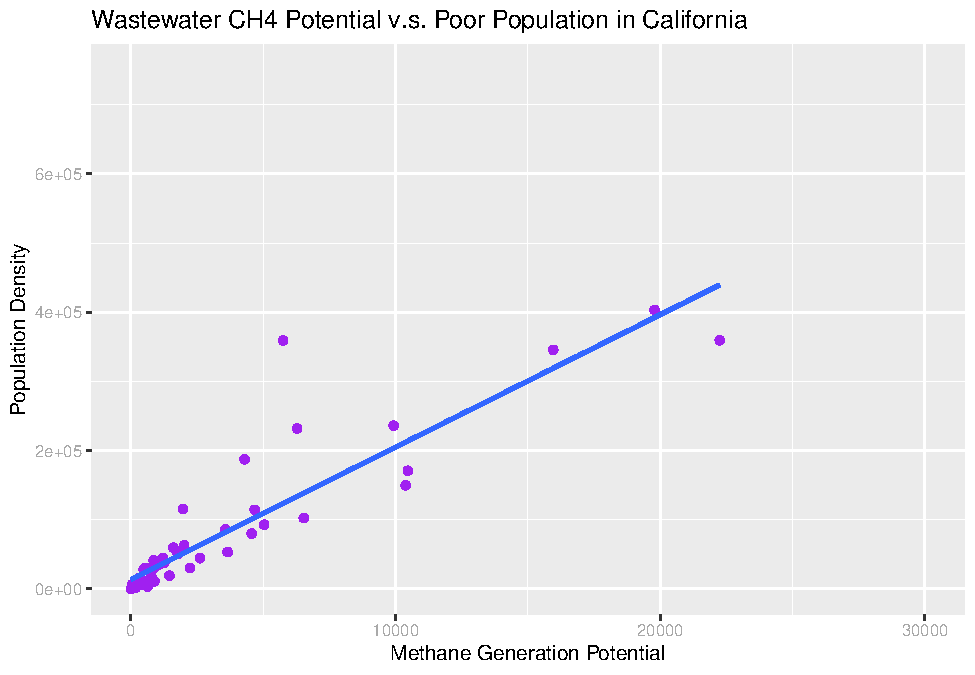
\includegraphics{FDR_ProjectReport_files/figure-latex/unnamed-chunk-8-3.pdf}
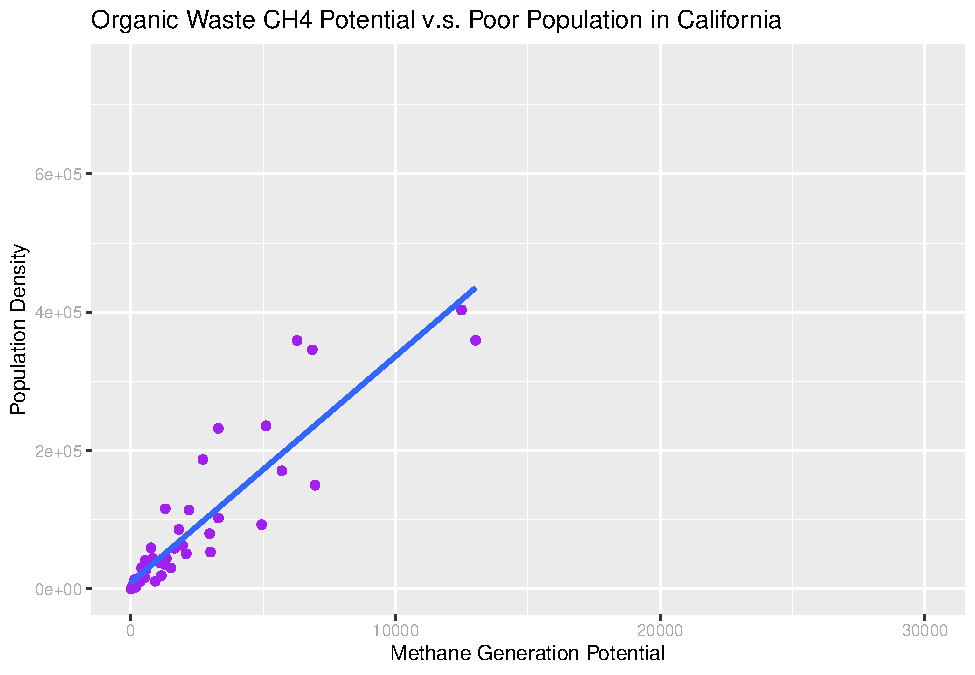
\includegraphics{FDR_ProjectReport_files/figure-latex/unnamed-chunk-8-4.pdf}
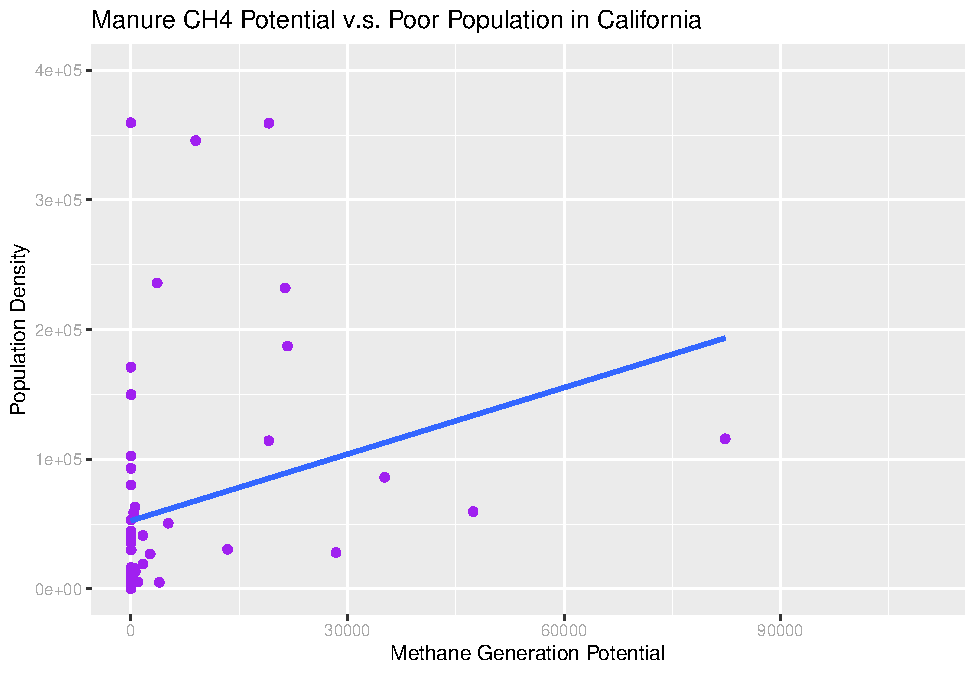
\includegraphics{FDR_ProjectReport_files/figure-latex/unnamed-chunk-8-5.pdf}

\newpage

\hypertarget{conclusion}{%
\section{Conclusion}\label{conclusion}}

Overall, the analysis conducted show that biogas generation potential
across counties in California is positively correlated with the
population density. This implies that the higher the population in a
specific area, the higher the biogas generation potential. However, the
analysis also recognises that generation potential and correlation with
population density varies according to the biomass source across
counties. As such, results show that animal based methane appeared to be
less correlated with population. Assumptions that best explain this
result are that more animals will contribute to animal-based biomass and
that human habitation is often less where animal population is dense.
Results of our analysis also show that the potential of landfill-based
biogas was not limited to densely or sparsely populated areas, while
organic waste and waste water represented the most significant sources
of biogas generation potential across California.

Future analysis can focus on improving the model presented in this
report by eliminating some outliers and using more recent datasets. This
study made use of older data sets because those were the ones most
recently made available on open and credible data portals. Other areas
of future analysis include exploring the level and process of
utilization of California's biogas generation potential, as well as how
utilization can be scaled. For example, the potential of leveraging the
biogas generation potential by enabling counties with lower generation
potentials to tap into the resources for those with higher
generation.This also includes scoping the potential to utilize biogas
energy for base load power or peaking, using various analyses including
a cost-benefit analysis.

\newpage

\hypertarget{references}{%
\section{References}\label{references}}

\textless add references here if relevant, otherwise delete this
section\textgreater{}

\end{document}
